\documentclass[a4paper]{article}
\usepackage{fullpage, array, graphicx}

\begin{document}
\title{G52SOF - Use Case Analysis}
\author{Harry Coupe, PSYHC5, 4321806}
\maketitle
\pagebreak

\section*{\underline{Use Case Scenario}}
\textbf{Use Case:} Adding deadline to calendar\\

\noindent\textbf{Primary Actors:}
\begin{itemize}
	\item Student User
	\item Teacher User
\end{itemize}

\noindent\textbf{Goal:} To add a deadline event to the calendar section of the app\\
\textbf{Preconditions:}
\begin{itemize}
	\item User has an account setup 
	\item User has a deadline to add to the calendar
\end{itemize}
\textbf{Main Success Scenario:}


\noindent\begin{tabular}{|m{0.7cm}|m{7.5cm}|m{0.7cm}|m{7.5cm}|}
	\hline
	\textbf{Step} & \textbf{Actor Action} & \textbf{Step} & \textbf{System Reaction} \\
	\hline
	1 & User selects a date from the calendar & 2 & The app comes to a single date view to allow event editing \\
	\hline
	3 & User selects add deadline option from single date view & 4 & Systems asks for deadline details e.g. Time, Class, Alerts etc..\\
	\hline
	5 & User enters deadline data & 6 & System asks user to verify deadline data is correct \\
	\hline
	7a & User verifies data is correct & 8a & System returns to main calendar view\\
	\hline
	7b & User selects the data is incorrect & 8b & System returns to single date view to allow event editing\\
	\hline
\end{tabular}



\noindent\textbf{Post Conditions:}
\begin{enumerate}
	\item The deadline is now added to the users calendar with the correct data
	\item The app returns to the calendar view
	\item The deadline is viewable and editable in the single date view
\end{enumerate}

\noindent\textbf{Exception Flows:}\\
\textbf{User selects an invalid date}\\
\noindent\begin{tabular}{|m{0.7cm}|m{7.5cm}|m{0.7cm}|m{7.5cm}|}
	\hline
	\textbf{Step} & \textbf{Actor Action} & \textbf{Step} & \textbf{System Reaction} \\
	\hline
	1 & User selects a date in the past, an invalid date & 2 & Systems shows an error "date chosen is invalid"\\
	\hline
	3 & User presses ok on the system error & 4 & System returns to the calendar view\\
	\hline
\end{tabular}
\\
\\
\textbf{Data entered is missing key data}\\
\noindent\begin{tabular}{|m{0.7cm}|m{7.5cm}|m{0.7cm}|m{7.5cm}|}
	\hline
	\textbf{Step} & \textbf{Actor Action} & \textbf{Step} & \textbf{System Reaction} \\
	\hline
	1 & User selects a date from the calendar & 2 & The app comes to a single date view to allow event editing \\
	\hline
	3 & User selects add deadline option from single date view & 4 & Systems asks for deadline details e.g. Time, Class, Alerts etc..\\
	\hline
	5 & User enters insufficient deadline data missing required fields & 6 & System shows an error "missing required fields" and returns to the deadline data view\\
	\hline
	7 & User enters sufficient deadline data & 8 & System asks user to verify deadline data is correct \\
	\hline
	9a & User verifies data is correct & 10a & System returns to main calendar view\\
	\hline
	9b & User selects the data is incorrect & 10b & System returns to single date view to allow event editing\\
	\hline
\end{tabular}
\pagebreak

\noindent\textbf{Failure to confirm or cancel data}\\
\noindent\begin{tabular}{|m{0.7cm}|m{7.5cm}|m{0.7cm}|m{7.5cm}|}
	\hline
	\textbf{Step} & \textbf{Actor Action} & \textbf{Step} & \textbf{System Reaction} \\
	\hline
	1 & User selects a date from the calendar & 2 & The app comes to a single date view to allow event editing \\
	\hline
	3 & User selects add deadline option from single date view & 4 & Systems asks for deadline details e.g. Time, Class, Alerts etc..\\
	\hline
	7 & User enters sufficient deadline data & 8 & System asks user to verify deadline data is correct \\
	\hline
	9 & User fails to confirm if data is correct & 10 & After 1 minute of inactivity the system returns to the single date view to wait for further editing\\
	\hline

\end{tabular}

\section*{\underline{Use Case Diagram}}
Below you will find in figure 1 the use case diagram of the features included in the calendar section of the app.
\begin{figure}[h!]
	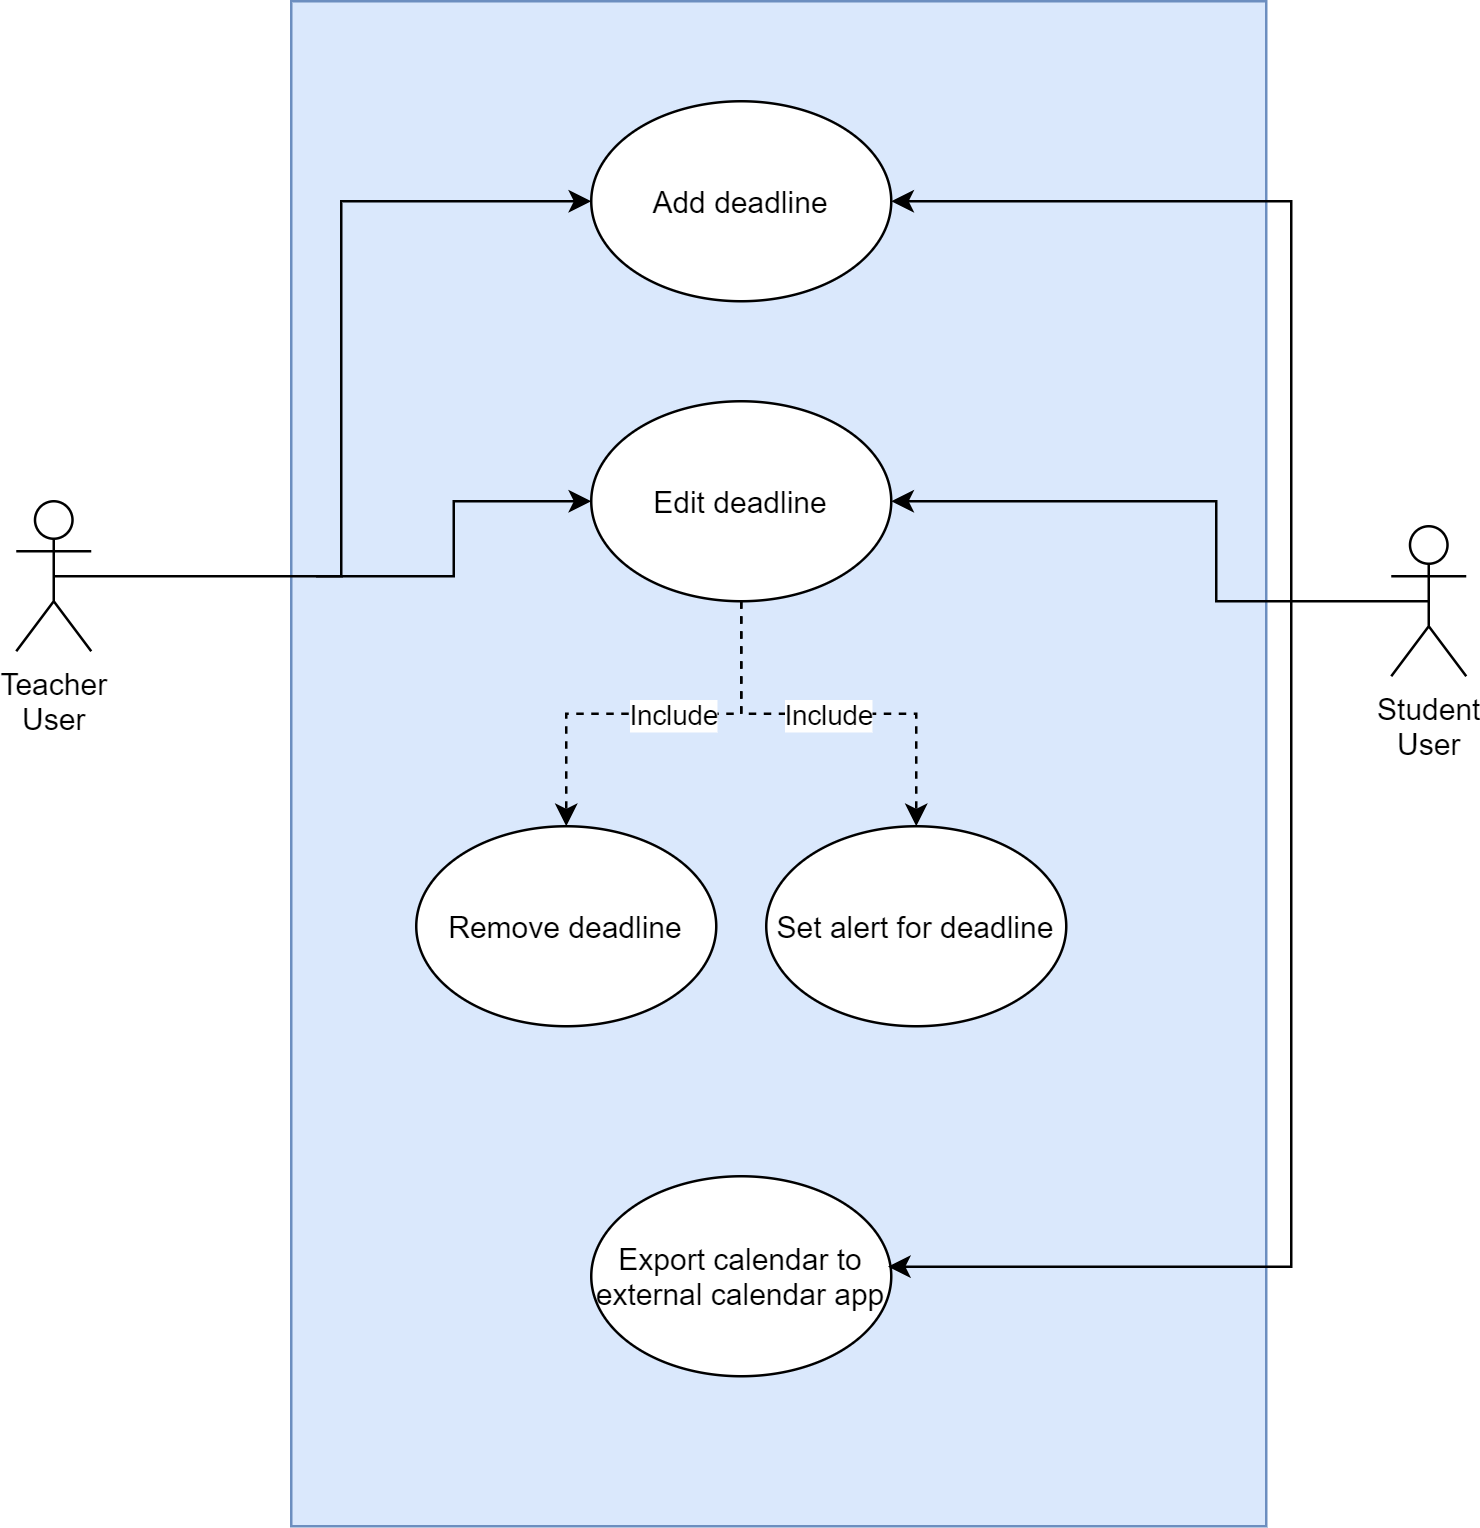
\includegraphics[scale=0.3]{UseCaseDiagram.png}
	\caption{Use Case Diagram of the calendar section of the app}
	\label{fig:Use Case Diagram}
\end{figure}


\pagebreak
\end{document}